\documentclass[11pt]{article}

    \usepackage[breakable]{tcolorbox}
    \usepackage{parskip} % Stop auto-indenting (to mimic markdown behaviour)
    

    % Basic figure setup, for now with no caption control since it's done
    % automatically by Pandoc (which extracts ![](path) syntax from Markdown).
    \usepackage{graphicx}
    % Maintain compatibility with old templates. Remove in nbconvert 6.0
    \let\Oldincludegraphics\includegraphics
    % Ensure that by default, figures have no caption (until we provide a
    % proper Figure object with a Caption API and a way to capture that
    % in the conversion process - todo).
    \usepackage{caption}
    \DeclareCaptionFormat{nocaption}{}
    \captionsetup{format=nocaption,aboveskip=0pt,belowskip=0pt}

    \usepackage{float}
    \floatplacement{figure}{H} % forces figures to be placed at the correct location
    \usepackage{xcolor} % Allow colors to be defined
    \usepackage{enumerate} % Needed for markdown enumerations to work
    \usepackage{geometry} % Used to adjust the document margins
    \usepackage{amsmath} % Equations
    \usepackage{amssymb} % Equations
    \usepackage{textcomp} % defines textquotesingle
    % Hack from http://tex.stackexchange.com/a/47451/13684:
    \AtBeginDocument{%
        \def\PYZsq{\textquotesingle}% Upright quotes in Pygmentized code
    }
    \usepackage{upquote} % Upright quotes for verbatim code
    \usepackage{eurosym} % defines \euro

    \usepackage{iftex}
    \ifPDFTeX
        \usepackage[T1]{fontenc}
        \IfFileExists{alphabeta.sty}{
              \usepackage{alphabeta}
          }{
              \usepackage[mathletters]{ucs}
              \usepackage[utf8x]{inputenc}
          }
    \else
        \usepackage{fontspec}
        \usepackage{unicode-math}
    \fi

    \usepackage{fancyvrb} % verbatim replacement that allows latex
    \usepackage{grffile} % extends the file name processing of package graphics
                         % to support a larger range
    \makeatletter % fix for old versions of grffile with XeLaTeX
    \@ifpackagelater{grffile}{2019/11/01}
    {
      % Do nothing on new versions
    }
    {
      \def\Gread@@xetex#1{%
        \IfFileExists{"\Gin@base".bb}%
        {\Gread@eps{\Gin@base.bb}}%
        {\Gread@@xetex@aux#1}%
      }
    }
    \makeatother
    \usepackage[Export]{adjustbox} % Used to constrain images to a maximum size
    \adjustboxset{max size={0.9\linewidth}{0.9\paperheight}}

    % The hyperref package gives us a pdf with properly built
    % internal navigation ('pdf bookmarks' for the table of contents,
    % internal cross-reference links, web links for URLs, etc.)
    \usepackage{hyperref}
    % The default LaTeX title has an obnoxious amount of whitespace. By default,
    % titling removes some of it. It also provides customization options.
    \usepackage{titling}
    \usepackage{longtable} % longtable support required by pandoc >1.10
    \usepackage{booktabs}  % table support for pandoc > 1.12.2
    \usepackage{array}     % table support for pandoc >= 2.11.3
    \usepackage{calc}      % table minipage width calculation for pandoc >= 2.11.1
    \usepackage[inline]{enumitem} % IRkernel/repr support (it uses the enumerate* environment)
    \usepackage[normalem]{ulem} % ulem is needed to support strikethroughs (\sout)
                                % normalem makes italics be italics, not underlines
    \usepackage{mathrsfs}
    

    
    % Colors for the hyperref package
    \definecolor{urlcolor}{rgb}{0,.145,.698}
    \definecolor{linkcolor}{rgb}{.71,0.21,0.01}
    \definecolor{citecolor}{rgb}{.12,.54,.11}

    % ANSI colors
    \definecolor{ansi-black}{HTML}{3E424D}
    \definecolor{ansi-black-intense}{HTML}{282C36}
    \definecolor{ansi-red}{HTML}{E75C58}
    \definecolor{ansi-red-intense}{HTML}{B22B31}
    \definecolor{ansi-green}{HTML}{00A250}
    \definecolor{ansi-green-intense}{HTML}{007427}
    \definecolor{ansi-yellow}{HTML}{DDB62B}
    \definecolor{ansi-yellow-intense}{HTML}{B27D12}
    \definecolor{ansi-blue}{HTML}{208FFB}
    \definecolor{ansi-blue-intense}{HTML}{0065CA}
    \definecolor{ansi-magenta}{HTML}{D160C4}
    \definecolor{ansi-magenta-intense}{HTML}{A03196}
    \definecolor{ansi-cyan}{HTML}{60C6C8}
    \definecolor{ansi-cyan-intense}{HTML}{258F8F}
    \definecolor{ansi-white}{HTML}{C5C1B4}
    \definecolor{ansi-white-intense}{HTML}{A1A6B2}
    \definecolor{ansi-default-inverse-fg}{HTML}{FFFFFF}
    \definecolor{ansi-default-inverse-bg}{HTML}{000000}

    % common color for the border for error outputs.
    \definecolor{outerrorbackground}{HTML}{FFDFDF}

    % commands and environments needed by pandoc snippets
    % extracted from the output of `pandoc -s`
    \providecommand{\tightlist}{%
      \setlength{\itemsep}{0pt}\setlength{\parskip}{0pt}}
    \DefineVerbatimEnvironment{Highlighting}{Verbatim}{commandchars=\\\{\}}
    % Add ',fontsize=\small' for more characters per line
    \newenvironment{Shaded}{}{}
    \newcommand{\KeywordTok}[1]{\textcolor[rgb]{0.00,0.44,0.13}{\textbf{{#1}}}}
    \newcommand{\DataTypeTok}[1]{\textcolor[rgb]{0.56,0.13,0.00}{{#1}}}
    \newcommand{\DecValTok}[1]{\textcolor[rgb]{0.25,0.63,0.44}{{#1}}}
    \newcommand{\BaseNTok}[1]{\textcolor[rgb]{0.25,0.63,0.44}{{#1}}}
    \newcommand{\FloatTok}[1]{\textcolor[rgb]{0.25,0.63,0.44}{{#1}}}
    \newcommand{\CharTok}[1]{\textcolor[rgb]{0.25,0.44,0.63}{{#1}}}
    \newcommand{\StringTok}[1]{\textcolor[rgb]{0.25,0.44,0.63}{{#1}}}
    \newcommand{\CommentTok}[1]{\textcolor[rgb]{0.38,0.63,0.69}{\textit{{#1}}}}
    \newcommand{\OtherTok}[1]{\textcolor[rgb]{0.00,0.44,0.13}{{#1}}}
    \newcommand{\AlertTok}[1]{\textcolor[rgb]{1.00,0.00,0.00}{\textbf{{#1}}}}
    \newcommand{\FunctionTok}[1]{\textcolor[rgb]{0.02,0.16,0.49}{{#1}}}
    \newcommand{\RegionMarkerTok}[1]{{#1}}
    \newcommand{\ErrorTok}[1]{\textcolor[rgb]{1.00,0.00,0.00}{\textbf{{#1}}}}
    \newcommand{\NormalTok}[1]{{#1}}

    % Additional commands for more recent versions of Pandoc
    \newcommand{\ConstantTok}[1]{\textcolor[rgb]{0.53,0.00,0.00}{{#1}}}
    \newcommand{\SpecialCharTok}[1]{\textcolor[rgb]{0.25,0.44,0.63}{{#1}}}
    \newcommand{\VerbatimStringTok}[1]{\textcolor[rgb]{0.25,0.44,0.63}{{#1}}}
    \newcommand{\SpecialStringTok}[1]{\textcolor[rgb]{0.73,0.40,0.53}{{#1}}}
    \newcommand{\ImportTok}[1]{{#1}}
    \newcommand{\DocumentationTok}[1]{\textcolor[rgb]{0.73,0.13,0.13}{\textit{{#1}}}}
    \newcommand{\AnnotationTok}[1]{\textcolor[rgb]{0.38,0.63,0.69}{\textbf{\textit{{#1}}}}}
    \newcommand{\CommentVarTok}[1]{\textcolor[rgb]{0.38,0.63,0.69}{\textbf{\textit{{#1}}}}}
    \newcommand{\VariableTok}[1]{\textcolor[rgb]{0.10,0.09,0.49}{{#1}}}
    \newcommand{\ControlFlowTok}[1]{\textcolor[rgb]{0.00,0.44,0.13}{\textbf{{#1}}}}
    \newcommand{\OperatorTok}[1]{\textcolor[rgb]{0.40,0.40,0.40}{{#1}}}
    \newcommand{\BuiltInTok}[1]{{#1}}
    \newcommand{\ExtensionTok}[1]{{#1}}
    \newcommand{\PreprocessorTok}[1]{\textcolor[rgb]{0.74,0.48,0.00}{{#1}}}
    \newcommand{\AttributeTok}[1]{\textcolor[rgb]{0.49,0.56,0.16}{{#1}}}
    \newcommand{\InformationTok}[1]{\textcolor[rgb]{0.38,0.63,0.69}{\textbf{\textit{{#1}}}}}
    \newcommand{\WarningTok}[1]{\textcolor[rgb]{0.38,0.63,0.69}{\textbf{\textit{{#1}}}}}


    % Define a nice break command that doesn't care if a line doesn't already
    % exist.
    \def\br{\hspace*{\fill} \\* }
    % Math Jax compatibility definitions
    \def\gt{>}
    \def\lt{<}
    \let\Oldtex\TeX
    \let\Oldlatex\LaTeX
    \renewcommand{\TeX}{\textrm{\Oldtex}}
    \renewcommand{\LaTeX}{\textrm{\Oldlatex}}
    % Document parameters
    % Document title
    \title{lab1}
    
    
    
    
    
% Pygments definitions
\makeatletter
\def\PY@reset{\let\PY@it=\relax \let\PY@bf=\relax%
    \let\PY@ul=\relax \let\PY@tc=\relax%
    \let\PY@bc=\relax \let\PY@ff=\relax}
\def\PY@tok#1{\csname PY@tok@#1\endcsname}
\def\PY@toks#1+{\ifx\relax#1\empty\else%
    \PY@tok{#1}\expandafter\PY@toks\fi}
\def\PY@do#1{\PY@bc{\PY@tc{\PY@ul{%
    \PY@it{\PY@bf{\PY@ff{#1}}}}}}}
\def\PY#1#2{\PY@reset\PY@toks#1+\relax+\PY@do{#2}}

\@namedef{PY@tok@w}{\def\PY@tc##1{\textcolor[rgb]{0.73,0.73,0.73}{##1}}}
\@namedef{PY@tok@c}{\let\PY@it=\textit\def\PY@tc##1{\textcolor[rgb]{0.24,0.48,0.48}{##1}}}
\@namedef{PY@tok@cp}{\def\PY@tc##1{\textcolor[rgb]{0.61,0.40,0.00}{##1}}}
\@namedef{PY@tok@k}{\let\PY@bf=\textbf\def\PY@tc##1{\textcolor[rgb]{0.00,0.50,0.00}{##1}}}
\@namedef{PY@tok@kp}{\def\PY@tc##1{\textcolor[rgb]{0.00,0.50,0.00}{##1}}}
\@namedef{PY@tok@kt}{\def\PY@tc##1{\textcolor[rgb]{0.69,0.00,0.25}{##1}}}
\@namedef{PY@tok@o}{\def\PY@tc##1{\textcolor[rgb]{0.40,0.40,0.40}{##1}}}
\@namedef{PY@tok@ow}{\let\PY@bf=\textbf\def\PY@tc##1{\textcolor[rgb]{0.67,0.13,1.00}{##1}}}
\@namedef{PY@tok@nb}{\def\PY@tc##1{\textcolor[rgb]{0.00,0.50,0.00}{##1}}}
\@namedef{PY@tok@nf}{\def\PY@tc##1{\textcolor[rgb]{0.00,0.00,1.00}{##1}}}
\@namedef{PY@tok@nc}{\let\PY@bf=\textbf\def\PY@tc##1{\textcolor[rgb]{0.00,0.00,1.00}{##1}}}
\@namedef{PY@tok@nn}{\let\PY@bf=\textbf\def\PY@tc##1{\textcolor[rgb]{0.00,0.00,1.00}{##1}}}
\@namedef{PY@tok@ne}{\let\PY@bf=\textbf\def\PY@tc##1{\textcolor[rgb]{0.80,0.25,0.22}{##1}}}
\@namedef{PY@tok@nv}{\def\PY@tc##1{\textcolor[rgb]{0.10,0.09,0.49}{##1}}}
\@namedef{PY@tok@no}{\def\PY@tc##1{\textcolor[rgb]{0.53,0.00,0.00}{##1}}}
\@namedef{PY@tok@nl}{\def\PY@tc##1{\textcolor[rgb]{0.46,0.46,0.00}{##1}}}
\@namedef{PY@tok@ni}{\let\PY@bf=\textbf\def\PY@tc##1{\textcolor[rgb]{0.44,0.44,0.44}{##1}}}
\@namedef{PY@tok@na}{\def\PY@tc##1{\textcolor[rgb]{0.41,0.47,0.13}{##1}}}
\@namedef{PY@tok@nt}{\let\PY@bf=\textbf\def\PY@tc##1{\textcolor[rgb]{0.00,0.50,0.00}{##1}}}
\@namedef{PY@tok@nd}{\def\PY@tc##1{\textcolor[rgb]{0.67,0.13,1.00}{##1}}}
\@namedef{PY@tok@s}{\def\PY@tc##1{\textcolor[rgb]{0.73,0.13,0.13}{##1}}}
\@namedef{PY@tok@sd}{\let\PY@it=\textit\def\PY@tc##1{\textcolor[rgb]{0.73,0.13,0.13}{##1}}}
\@namedef{PY@tok@si}{\let\PY@bf=\textbf\def\PY@tc##1{\textcolor[rgb]{0.64,0.35,0.47}{##1}}}
\@namedef{PY@tok@se}{\let\PY@bf=\textbf\def\PY@tc##1{\textcolor[rgb]{0.67,0.36,0.12}{##1}}}
\@namedef{PY@tok@sr}{\def\PY@tc##1{\textcolor[rgb]{0.64,0.35,0.47}{##1}}}
\@namedef{PY@tok@ss}{\def\PY@tc##1{\textcolor[rgb]{0.10,0.09,0.49}{##1}}}
\@namedef{PY@tok@sx}{\def\PY@tc##1{\textcolor[rgb]{0.00,0.50,0.00}{##1}}}
\@namedef{PY@tok@m}{\def\PY@tc##1{\textcolor[rgb]{0.40,0.40,0.40}{##1}}}
\@namedef{PY@tok@gh}{\let\PY@bf=\textbf\def\PY@tc##1{\textcolor[rgb]{0.00,0.00,0.50}{##1}}}
\@namedef{PY@tok@gu}{\let\PY@bf=\textbf\def\PY@tc##1{\textcolor[rgb]{0.50,0.00,0.50}{##1}}}
\@namedef{PY@tok@gd}{\def\PY@tc##1{\textcolor[rgb]{0.63,0.00,0.00}{##1}}}
\@namedef{PY@tok@gi}{\def\PY@tc##1{\textcolor[rgb]{0.00,0.52,0.00}{##1}}}
\@namedef{PY@tok@gr}{\def\PY@tc##1{\textcolor[rgb]{0.89,0.00,0.00}{##1}}}
\@namedef{PY@tok@ge}{\let\PY@it=\textit}
\@namedef{PY@tok@gs}{\let\PY@bf=\textbf}
\@namedef{PY@tok@gp}{\let\PY@bf=\textbf\def\PY@tc##1{\textcolor[rgb]{0.00,0.00,0.50}{##1}}}
\@namedef{PY@tok@go}{\def\PY@tc##1{\textcolor[rgb]{0.44,0.44,0.44}{##1}}}
\@namedef{PY@tok@gt}{\def\PY@tc##1{\textcolor[rgb]{0.00,0.27,0.87}{##1}}}
\@namedef{PY@tok@err}{\def\PY@bc##1{{\setlength{\fboxsep}{\string -\fboxrule}\fcolorbox[rgb]{1.00,0.00,0.00}{1,1,1}{\strut ##1}}}}
\@namedef{PY@tok@kc}{\let\PY@bf=\textbf\def\PY@tc##1{\textcolor[rgb]{0.00,0.50,0.00}{##1}}}
\@namedef{PY@tok@kd}{\let\PY@bf=\textbf\def\PY@tc##1{\textcolor[rgb]{0.00,0.50,0.00}{##1}}}
\@namedef{PY@tok@kn}{\let\PY@bf=\textbf\def\PY@tc##1{\textcolor[rgb]{0.00,0.50,0.00}{##1}}}
\@namedef{PY@tok@kr}{\let\PY@bf=\textbf\def\PY@tc##1{\textcolor[rgb]{0.00,0.50,0.00}{##1}}}
\@namedef{PY@tok@bp}{\def\PY@tc##1{\textcolor[rgb]{0.00,0.50,0.00}{##1}}}
\@namedef{PY@tok@fm}{\def\PY@tc##1{\textcolor[rgb]{0.00,0.00,1.00}{##1}}}
\@namedef{PY@tok@vc}{\def\PY@tc##1{\textcolor[rgb]{0.10,0.09,0.49}{##1}}}
\@namedef{PY@tok@vg}{\def\PY@tc##1{\textcolor[rgb]{0.10,0.09,0.49}{##1}}}
\@namedef{PY@tok@vi}{\def\PY@tc##1{\textcolor[rgb]{0.10,0.09,0.49}{##1}}}
\@namedef{PY@tok@vm}{\def\PY@tc##1{\textcolor[rgb]{0.10,0.09,0.49}{##1}}}
\@namedef{PY@tok@sa}{\def\PY@tc##1{\textcolor[rgb]{0.73,0.13,0.13}{##1}}}
\@namedef{PY@tok@sb}{\def\PY@tc##1{\textcolor[rgb]{0.73,0.13,0.13}{##1}}}
\@namedef{PY@tok@sc}{\def\PY@tc##1{\textcolor[rgb]{0.73,0.13,0.13}{##1}}}
\@namedef{PY@tok@dl}{\def\PY@tc##1{\textcolor[rgb]{0.73,0.13,0.13}{##1}}}
\@namedef{PY@tok@s2}{\def\PY@tc##1{\textcolor[rgb]{0.73,0.13,0.13}{##1}}}
\@namedef{PY@tok@sh}{\def\PY@tc##1{\textcolor[rgb]{0.73,0.13,0.13}{##1}}}
\@namedef{PY@tok@s1}{\def\PY@tc##1{\textcolor[rgb]{0.73,0.13,0.13}{##1}}}
\@namedef{PY@tok@mb}{\def\PY@tc##1{\textcolor[rgb]{0.40,0.40,0.40}{##1}}}
\@namedef{PY@tok@mf}{\def\PY@tc##1{\textcolor[rgb]{0.40,0.40,0.40}{##1}}}
\@namedef{PY@tok@mh}{\def\PY@tc##1{\textcolor[rgb]{0.40,0.40,0.40}{##1}}}
\@namedef{PY@tok@mi}{\def\PY@tc##1{\textcolor[rgb]{0.40,0.40,0.40}{##1}}}
\@namedef{PY@tok@il}{\def\PY@tc##1{\textcolor[rgb]{0.40,0.40,0.40}{##1}}}
\@namedef{PY@tok@mo}{\def\PY@tc##1{\textcolor[rgb]{0.40,0.40,0.40}{##1}}}
\@namedef{PY@tok@ch}{\let\PY@it=\textit\def\PY@tc##1{\textcolor[rgb]{0.24,0.48,0.48}{##1}}}
\@namedef{PY@tok@cm}{\let\PY@it=\textit\def\PY@tc##1{\textcolor[rgb]{0.24,0.48,0.48}{##1}}}
\@namedef{PY@tok@cpf}{\let\PY@it=\textit\def\PY@tc##1{\textcolor[rgb]{0.24,0.48,0.48}{##1}}}
\@namedef{PY@tok@c1}{\let\PY@it=\textit\def\PY@tc##1{\textcolor[rgb]{0.24,0.48,0.48}{##1}}}
\@namedef{PY@tok@cs}{\let\PY@it=\textit\def\PY@tc##1{\textcolor[rgb]{0.24,0.48,0.48}{##1}}}

\def\PYZbs{\char`\\}
\def\PYZus{\char`\_}
\def\PYZob{\char`\{}
\def\PYZcb{\char`\}}
\def\PYZca{\char`\^}
\def\PYZam{\char`\&}
\def\PYZlt{\char`\<}
\def\PYZgt{\char`\>}
\def\PYZsh{\char`\#}
\def\PYZpc{\char`\%}
\def\PYZdl{\char`\$}
\def\PYZhy{\char`\-}
\def\PYZsq{\char`\'}
\def\PYZdq{\char`\"}
\def\PYZti{\char`\~}
% for compatibility with earlier versions
\def\PYZat{@}
\def\PYZlb{[}
\def\PYZrb{]}
\makeatother


    % For linebreaks inside Verbatim environment from package fancyvrb.
    \makeatletter
        \newbox\Wrappedcontinuationbox
        \newbox\Wrappedvisiblespacebox
        \newcommand*\Wrappedvisiblespace {\textcolor{red}{\textvisiblespace}}
        \newcommand*\Wrappedcontinuationsymbol {\textcolor{red}{\llap{\tiny$\m@th\hookrightarrow$}}}
        \newcommand*\Wrappedcontinuationindent {3ex }
        \newcommand*\Wrappedafterbreak {\kern\Wrappedcontinuationindent\copy\Wrappedcontinuationbox}
        % Take advantage of the already applied Pygments mark-up to insert
        % potential linebreaks for TeX processing.
        %        {, <, #, %, $, ' and ": go to next line.
        %        _, }, ^, &, >, - and ~: stay at end of broken line.
        % Use of \textquotesingle for straight quote.
        \newcommand*\Wrappedbreaksatspecials {%
            \def\PYGZus{\discretionary{\char`\_}{\Wrappedafterbreak}{\char`\_}}%
            \def\PYGZob{\discretionary{}{\Wrappedafterbreak\char`\{}{\char`\{}}%
            \def\PYGZcb{\discretionary{\char`\}}{\Wrappedafterbreak}{\char`\}}}%
            \def\PYGZca{\discretionary{\char`\^}{\Wrappedafterbreak}{\char`\^}}%
            \def\PYGZam{\discretionary{\char`\&}{\Wrappedafterbreak}{\char`\&}}%
            \def\PYGZlt{\discretionary{}{\Wrappedafterbreak\char`\<}{\char`\<}}%
            \def\PYGZgt{\discretionary{\char`\>}{\Wrappedafterbreak}{\char`\>}}%
            \def\PYGZsh{\discretionary{}{\Wrappedafterbreak\char`\#}{\char`\#}}%
            \def\PYGZpc{\discretionary{}{\Wrappedafterbreak\char`\%}{\char`\%}}%
            \def\PYGZdl{\discretionary{}{\Wrappedafterbreak\char`\$}{\char`\$}}%
            \def\PYGZhy{\discretionary{\char`\-}{\Wrappedafterbreak}{\char`\-}}%
            \def\PYGZsq{\discretionary{}{\Wrappedafterbreak\textquotesingle}{\textquotesingle}}%
            \def\PYGZdq{\discretionary{}{\Wrappedafterbreak\char`\"}{\char`\"}}%
            \def\PYGZti{\discretionary{\char`\~}{\Wrappedafterbreak}{\char`\~}}%
        }
        % Some characters . , ; ? ! / are not pygmentized.
        % This macro makes them "active" and they will insert potential linebreaks
        \newcommand*\Wrappedbreaksatpunct {%
            \lccode`\~`\.\lowercase{\def~}{\discretionary{\hbox{\char`\.}}{\Wrappedafterbreak}{\hbox{\char`\.}}}%
            \lccode`\~`\,\lowercase{\def~}{\discretionary{\hbox{\char`\,}}{\Wrappedafterbreak}{\hbox{\char`\,}}}%
            \lccode`\~`\;\lowercase{\def~}{\discretionary{\hbox{\char`\;}}{\Wrappedafterbreak}{\hbox{\char`\;}}}%
            \lccode`\~`\:\lowercase{\def~}{\discretionary{\hbox{\char`\:}}{\Wrappedafterbreak}{\hbox{\char`\:}}}%
            \lccode`\~`\?\lowercase{\def~}{\discretionary{\hbox{\char`\?}}{\Wrappedafterbreak}{\hbox{\char`\?}}}%
            \lccode`\~`\!\lowercase{\def~}{\discretionary{\hbox{\char`\!}}{\Wrappedafterbreak}{\hbox{\char`\!}}}%
            \lccode`\~`\/\lowercase{\def~}{\discretionary{\hbox{\char`\/}}{\Wrappedafterbreak}{\hbox{\char`\/}}}%
            \catcode`\.\active
            \catcode`\,\active
            \catcode`\;\active
            \catcode`\:\active
            \catcode`\?\active
            \catcode`\!\active
            \catcode`\/\active
            \lccode`\~`\~
        }
    \makeatother

    \let\OriginalVerbatim=\Verbatim
    \makeatletter
    \renewcommand{\Verbatim}[1][1]{%
        %\parskip\z@skip
        \sbox\Wrappedcontinuationbox {\Wrappedcontinuationsymbol}%
        \sbox\Wrappedvisiblespacebox {\FV@SetupFont\Wrappedvisiblespace}%
        \def\FancyVerbFormatLine ##1{\hsize\linewidth
            \vtop{\raggedright\hyphenpenalty\z@\exhyphenpenalty\z@
                \doublehyphendemerits\z@\finalhyphendemerits\z@
                \strut ##1\strut}%
        }%
        % If the linebreak is at a space, the latter will be displayed as visible
        % space at end of first line, and a continuation symbol starts next line.
        % Stretch/shrink are however usually zero for typewriter font.
        \def\FV@Space {%
            \nobreak\hskip\z@ plus\fontdimen3\font minus\fontdimen4\font
            \discretionary{\copy\Wrappedvisiblespacebox}{\Wrappedafterbreak}
            {\kern\fontdimen2\font}%
        }%

        % Allow breaks at special characters using \PYG... macros.
        \Wrappedbreaksatspecials
        % Breaks at punctuation characters . , ; ? ! and / need catcode=\active
        \OriginalVerbatim[#1,codes*=\Wrappedbreaksatpunct]%
    }
    \makeatother

    % Exact colors from NB
    \definecolor{incolor}{HTML}{303F9F}
    \definecolor{outcolor}{HTML}{D84315}
    \definecolor{cellborder}{HTML}{CFCFCF}
    \definecolor{cellbackground}{HTML}{F7F7F7}

    % prompt
    \makeatletter
    \newcommand{\boxspacing}{\kern\kvtcb@left@rule\kern\kvtcb@boxsep}
    \makeatother
    \newcommand{\prompt}[4]{
        {\ttfamily\llap{{\color{#2}[#3]:\hspace{3pt}#4}}\vspace{-\baselineskip}}
    }
    

    
    % Prevent overflowing lines due to hard-to-break entities
    \sloppy
    % Setup hyperref package
    \hypersetup{
      breaklinks=true,  % so long urls are correctly broken across lines
      colorlinks=true,
      urlcolor=urlcolor,
      linkcolor=linkcolor,
      citecolor=citecolor,
      }
    % Slightly bigger margins than the latex defaults
    
    \geometry{verbose,tmargin=1in,bmargin=1in,lmargin=1in,rmargin=1in}
    
    

\begin{document}
    
    \maketitle
    
    

    
    \section{Computer Vision Lab 1 - Basic image
operations}\label{computer-vision-lab-1---basic-image-operations}

    Imports \& name-adding function

    \begin{tcolorbox}[breakable, size=fbox, boxrule=1pt, pad at break*=1mm,colback=cellbackground, colframe=cellborder]
\prompt{In}{incolor}{1}{\boxspacing}
\begin{Verbatim}[commandchars=\\\{\}]
\PY{k+kn}{import} \PY{n+nn}{cv2}
\PY{k+kn}{import} \PY{n+nn}{numpy} \PY{k}{as} \PY{n+nn}{np}

\PY{n}{NAME} \PY{o}{=} \PY{l+s+s2}{\PYZdq{}}\PY{l+s+s2}{Rens Delaplace}\PY{l+s+s2}{\PYZdq{}}

\PY{k}{def} \PY{n+nf}{add\PYZus{}name\PYZus{}to\PYZus{}image}\PY{p}{(}\PY{n}{image}\PY{p}{)}\PY{p}{:}
\PY{+w}{    }\PY{l+s+sd}{\PYZdq{}\PYZdq{}\PYZdq{}}
\PY{l+s+sd}{    Voeg de naam toe aan de afbeelding op een standaard positie (rechtsonder).}
\PY{l+s+sd}{    :param image: De afbeelding waarop de naam wordt toegevoegd.}
\PY{l+s+sd}{    :return: De afbeelding met de naam toegevoegd.}
\PY{l+s+sd}{    \PYZdq{}\PYZdq{}\PYZdq{}}
    \PY{n}{font} \PY{o}{=} \PY{n}{cv2}\PY{o}{.}\PY{n}{FONT\PYZus{}HERSHEY\PYZus{}SIMPLEX}
    \PY{n}{font\PYZus{}scale} \PY{o}{=} \PY{l+m+mf}{0.6}
    \PY{n}{thickness} \PY{o}{=} \PY{l+m+mi}{1}
    
    \PY{c+c1}{\PYZsh{} Bereken de grootte van de tekst}
    \PY{n}{text\PYZus{}size} \PY{o}{=} \PY{n}{cv2}\PY{o}{.}\PY{n}{getTextSize}\PY{p}{(}\PY{n}{NAME}\PY{p}{,} \PY{n}{font}\PY{p}{,} \PY{n}{font\PYZus{}scale}\PY{p}{,} \PY{n}{thickness}\PY{p}{)}\PY{p}{[}\PY{l+m+mi}{0}\PY{p}{]}
    
    \PY{c+c1}{\PYZsh{} Bepaal de positie rechtsonder}
    \PY{n}{position} \PY{o}{=} \PY{p}{(}\PY{n}{image}\PY{o}{.}\PY{n}{shape}\PY{p}{[}\PY{l+m+mi}{1}\PY{p}{]} \PY{o}{\PYZhy{}} \PY{n}{text\PYZus{}size}\PY{p}{[}\PY{l+m+mi}{0}\PY{p}{]} \PY{o}{\PYZhy{}} \PY{l+m+mi}{10}\PY{p}{,} \PY{n}{image}\PY{o}{.}\PY{n}{shape}\PY{p}{[}\PY{l+m+mi}{0}\PY{p}{]} \PY{o}{\PYZhy{}} \PY{l+m+mi}{10}\PY{p}{)}
    
    \PY{c+c1}{\PYZsh{} Voeg de naam toe aan de afbeelding}
    \PY{n}{cv2}\PY{o}{.}\PY{n}{putText}\PY{p}{(}\PY{n}{image}\PY{p}{,} \PY{n}{NAME}\PY{p}{,} \PY{n}{position}\PY{p}{,} \PY{n}{font}\PY{p}{,} \PY{n}{font\PYZus{}scale}\PY{p}{,} \PY{p}{(}\PY{l+m+mi}{255}\PY{p}{,} \PY{l+m+mi}{255}\PY{p}{,} \PY{l+m+mi}{255}\PY{p}{)}\PY{p}{,} \PY{n}{thickness}\PY{p}{,} \PY{n}{cv2}\PY{o}{.}\PY{n}{LINE\PYZus{}AA}\PY{p}{)}
    
    \PY{k}{return} \PY{n}{image}
\end{Verbatim}
\end{tcolorbox}

    \subsection{Reading, manipulating and writing pixel
data}\label{reading-manipulating-and-writing-pixel-data}

    \subsubsection{Exercise 1}\label{exercise-1}

    \begin{tcolorbox}[breakable, size=fbox, boxrule=1pt, pad at break*=1mm,colback=cellbackground, colframe=cellborder]
\prompt{In}{incolor}{2}{\boxspacing}
\begin{Verbatim}[commandchars=\\\{\}]
\PY{c+c1}{\PYZsh{} Read the image}
\PY{n}{image} \PY{o}{=} \PY{n}{cv2}\PY{o}{.}\PY{n}{imread}\PY{p}{(}\PY{l+s+s2}{\PYZdq{}}\PY{l+s+s2}{img/clouds.jpg}\PY{l+s+s2}{\PYZdq{}}\PY{p}{)}

\PY{c+c1}{\PYZsh{} dimensions}
\PY{n}{height}\PY{p}{,} \PY{n}{width}\PY{p}{,} \PY{n}{channels} \PY{o}{=} \PY{n}{image}\PY{o}{.}\PY{n}{shape}
\PY{n+nb}{print}\PY{p}{(}\PY{l+s+sa}{f}\PY{l+s+s2}{\PYZdq{}}\PY{l+s+s2}{Image dimensions: Height=}\PY{l+s+si}{\PYZob{}}\PY{n}{height}\PY{l+s+si}{\PYZcb{}}\PY{l+s+s2}{, Width=}\PY{l+s+si}{\PYZob{}}\PY{n}{width}\PY{l+s+si}{\PYZcb{}}\PY{l+s+s2}{, Channels=}\PY{l+s+si}{\PYZob{}}\PY{n}{channels}\PY{l+s+si}{\PYZcb{}}\PY{l+s+s2}{\PYZdq{}}\PY{p}{)}
\end{Verbatim}
\end{tcolorbox}

    \begin{Verbatim}[commandchars=\\\{\}]
Image dimensions: Height=360, Width=801, Channels=3
    \end{Verbatim}

    \paragraph{Question 1}\label{question-1}

    \begin{quote}
What do the dimensions of the image array represent?
\end{quote}

They represent the hight, width and color channels of the image.

    \paragraph{Assignment 1}\label{assignment-1}

\begin{quote}
Crop the image so it becomes square by chopping off the a part on the
right side.
\end{quote}

    \begin{tcolorbox}[breakable, size=fbox, boxrule=1pt, pad at break*=1mm,colback=cellbackground, colframe=cellborder]
\prompt{In}{incolor}{3}{\boxspacing}
\begin{Verbatim}[commandchars=\\\{\}]
\PY{n}{square\PYZus{}size} \PY{o}{=} \PY{n+nb}{min}\PY{p}{(}\PY{n}{height}\PY{p}{,} \PY{n}{width}\PY{p}{)}
\PY{n}{cropped\PYZus{}image} \PY{o}{=} \PY{n}{image}\PY{p}{[}\PY{p}{:}\PY{p}{,} \PY{p}{:}\PY{n}{square\PYZus{}size}\PY{p}{]}

\PY{n}{cropped\PYZus{}image} \PY{o}{=} \PY{n}{add\PYZus{}name\PYZus{}to\PYZus{}image}\PY{p}{(}\PY{n}{cropped\PYZus{}image}\PY{p}{)}
\PY{n}{cv2}\PY{o}{.}\PY{n}{imwrite}\PY{p}{(}\PY{l+s+s1}{\PYZsq{}}\PY{l+s+s1}{out/assignement1.jpg}\PY{l+s+s1}{\PYZsq{}}\PY{p}{,} \PY{n}{cropped\PYZus{}image}\PY{p}{)}
\end{Verbatim}
\end{tcolorbox}

            \begin{tcolorbox}[breakable, size=fbox, boxrule=.5pt, pad at break*=1mm, opacityfill=0]
\prompt{Out}{outcolor}{3}{\boxspacing}
\begin{Verbatim}[commandchars=\\\{\}]
True
\end{Verbatim}
\end{tcolorbox}
        
    \begin{figure}
\centering
\pandocbounded{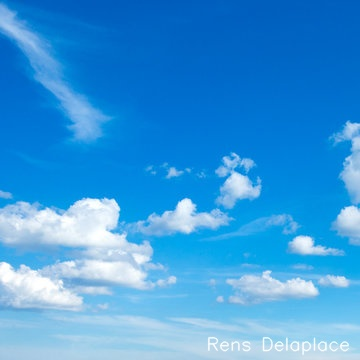
\includegraphics[keepaspectratio]{./out/assignement1.jpg}}
\caption{alt text}
\end{figure}

    \paragraph{Assignment 2}\label{assignment-2}

\begin{quote}
Discolor the image by reducing the intensity of the red value of every
pixel by half.
\end{quote}

    \begin{tcolorbox}[breakable, size=fbox, boxrule=1pt, pad at break*=1mm,colback=cellbackground, colframe=cellborder]
\prompt{In}{incolor}{4}{\boxspacing}
\begin{Verbatim}[commandchars=\\\{\}]
\PY{c+c1}{\PYZsh{} Assignment 2: Reduce the red intensity by half}
\PY{n}{red\PYZus{}reduced} \PY{o}{=} \PY{n}{image}\PY{o}{.}\PY{n}{copy}\PY{p}{(}\PY{p}{)}
\PY{n}{red\PYZus{}reduced}\PY{p}{[}\PY{p}{:}\PY{p}{,} \PY{p}{:}\PY{p}{,} \PY{l+m+mi}{2}\PY{p}{]} \PY{o}{=} \PY{n}{red\PYZus{}reduced}\PY{p}{[}\PY{p}{:}\PY{p}{,} \PY{p}{:}\PY{p}{,} \PY{l+m+mi}{2}\PY{p}{]} \PY{o}{/}\PY{o}{/} \PY{l+m+mi}{2}  \PY{c+c1}{\PYZsh{} OpenCV uses BGR format}
\PY{n}{red\PYZus{}reduced} \PY{o}{=} \PY{n}{add\PYZus{}name\PYZus{}to\PYZus{}image}\PY{p}{(}\PY{n}{red\PYZus{}reduced}\PY{p}{)}
\PY{n}{cv2}\PY{o}{.}\PY{n}{imwrite}\PY{p}{(}\PY{l+s+s1}{\PYZsq{}}\PY{l+s+s1}{out/assignement2.jpg}\PY{l+s+s1}{\PYZsq{}}\PY{p}{,} \PY{n}{red\PYZus{}reduced}\PY{p}{)}
\end{Verbatim}
\end{tcolorbox}

            \begin{tcolorbox}[breakable, size=fbox, boxrule=.5pt, pad at break*=1mm, opacityfill=0]
\prompt{Out}{outcolor}{4}{\boxspacing}
\begin{Verbatim}[commandchars=\\\{\}]
True
\end{Verbatim}
\end{tcolorbox}
        
    \begin{figure}
\centering
\pandocbounded{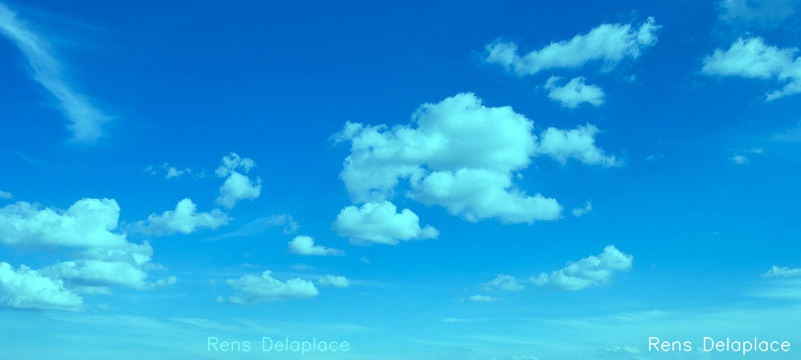
\includegraphics[keepaspectratio]{./out/assignement2.jpg}}
\caption{alt text}
\end{figure}

    \paragraph{Assignment 3}\label{assignment-3}

\begin{quote}
Discolor the image by doubling the intensity of the red value of every
pixel. You may have to handle an overflow problem (and use two more
lines of code).
\end{quote}

    \begin{tcolorbox}[breakable, size=fbox, boxrule=1pt, pad at break*=1mm,colback=cellbackground, colframe=cellborder]
\prompt{In}{incolor}{5}{\boxspacing}
\begin{Verbatim}[commandchars=\\\{\}]
\PY{n}{red\PYZus{}doubled} \PY{o}{=} \PY{n}{image}\PY{o}{.}\PY{n}{copy}\PY{p}{(}\PY{p}{)}
\PY{n}{red\PYZus{}doubled}\PY{p}{[}\PY{p}{:}\PY{p}{,} \PY{p}{:}\PY{p}{,} \PY{l+m+mi}{2}\PY{p}{]} \PY{o}{=} \PY{n}{np}\PY{o}{.}\PY{n}{clip}\PY{p}{(}\PY{n}{red\PYZus{}doubled}\PY{p}{[}\PY{p}{:}\PY{p}{,} \PY{p}{:}\PY{p}{,} \PY{l+m+mi}{2}\PY{p}{]} \PY{o}{*} \PY{l+m+mi}{2}\PY{p}{,} \PY{l+m+mi}{0}\PY{p}{,} \PY{l+m+mi}{255}\PY{p}{)}

\PY{n}{red\PYZus{}doubled} \PY{o}{=} \PY{n}{add\PYZus{}name\PYZus{}to\PYZus{}image}\PY{p}{(}\PY{n}{red\PYZus{}doubled}\PY{p}{)}
\PY{n}{cv2}\PY{o}{.}\PY{n}{imwrite}\PY{p}{(}\PY{l+s+s1}{\PYZsq{}}\PY{l+s+s1}{out/assignement3.jpg}\PY{l+s+s1}{\PYZsq{}}\PY{p}{,} \PY{n}{red\PYZus{}doubled}\PY{p}{)}
\end{Verbatim}
\end{tcolorbox}

            \begin{tcolorbox}[breakable, size=fbox, boxrule=.5pt, pad at break*=1mm, opacityfill=0]
\prompt{Out}{outcolor}{5}{\boxspacing}
\begin{Verbatim}[commandchars=\\\{\}]
True
\end{Verbatim}
\end{tcolorbox}
        
    \begin{figure}
\centering
\pandocbounded{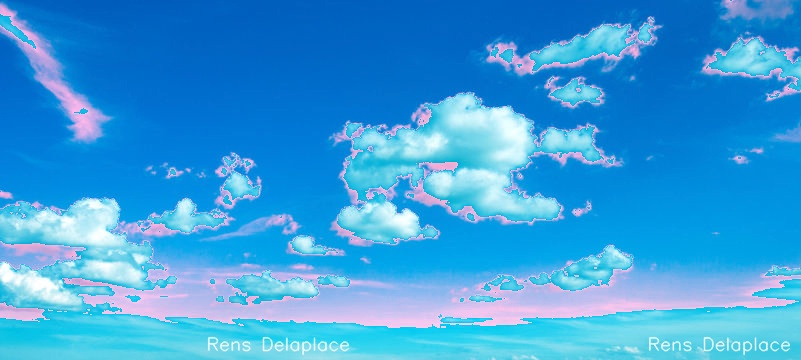
\includegraphics[keepaspectratio]{./out/assignement3.jpg}}
\caption{alt text}
\end{figure}

    \paragraph{Assignment 4}\label{assignment-4}

\begin{quote}
Make a regular grid of black dots on the image so that the dots are 10
pixels apart vertically and horizontally.
\end{quote}

    \begin{tcolorbox}[breakable, size=fbox, boxrule=1pt, pad at break*=1mm,colback=cellbackground, colframe=cellborder]
\prompt{In}{incolor}{6}{\boxspacing}
\begin{Verbatim}[commandchars=\\\{\}]
\PY{n}{grid\PYZus{}image} \PY{o}{=} \PY{n}{image}\PY{o}{.}\PY{n}{copy}\PY{p}{(}\PY{p}{)}
\PY{k}{for} \PY{n}{y} \PY{o+ow}{in} \PY{n+nb}{range}\PY{p}{(}\PY{l+m+mi}{0}\PY{p}{,} \PY{n}{height}\PY{p}{,} \PY{l+m+mi}{10}\PY{p}{)}\PY{p}{:}
    \PY{k}{for} \PY{n}{x} \PY{o+ow}{in} \PY{n+nb}{range}\PY{p}{(}\PY{l+m+mi}{0}\PY{p}{,} \PY{n}{width}\PY{p}{,} \PY{l+m+mi}{10}\PY{p}{)}\PY{p}{:}
        \PY{n}{cv2}\PY{o}{.}\PY{n}{circle}\PY{p}{(}\PY{n}{grid\PYZus{}image}\PY{p}{,} \PY{p}{(}\PY{n}{x}\PY{p}{,} \PY{n}{y}\PY{p}{)}\PY{p}{,} \PY{l+m+mi}{1}\PY{p}{,} \PY{p}{(}\PY{l+m+mi}{0}\PY{p}{,} \PY{l+m+mi}{0}\PY{p}{,} \PY{l+m+mi}{0}\PY{p}{)}\PY{p}{,} \PY{o}{\PYZhy{}}\PY{l+m+mi}{1}\PY{p}{)}  \PY{c+c1}{\PYZsh{} Black dot }
        \PY{c+c1}{\PYZsh{} (grid\PYZus{}image → The image on which to draw}
        \PY{c+c1}{\PYZsh{} (x, y) → The position of the center of the circle. }
        \PY{c+c1}{\PYZsh{} 2 → Radius of the circle (2 pixels)}
        \PY{c+c1}{\PYZsh{} (0, 0, 0) → Black color in BGR format.}
        \PY{c+c1}{\PYZsh{} \PYZhy{}1 → Fills the circle completely.}
        
\PY{n}{grid\PYZus{}image} \PY{o}{=} \PY{n}{add\PYZus{}name\PYZus{}to\PYZus{}image}\PY{p}{(}\PY{n}{grid\PYZus{}image}\PY{p}{)}
\PY{n}{cv2}\PY{o}{.}\PY{n}{imwrite}\PY{p}{(}\PY{l+s+s1}{\PYZsq{}}\PY{l+s+s1}{out/assignement4.jpg}\PY{l+s+s1}{\PYZsq{}}\PY{p}{,} \PY{n}{grid\PYZus{}image}\PY{p}{)}
\end{Verbatim}
\end{tcolorbox}

            \begin{tcolorbox}[breakable, size=fbox, boxrule=.5pt, pad at break*=1mm, opacityfill=0]
\prompt{Out}{outcolor}{6}{\boxspacing}
\begin{Verbatim}[commandchars=\\\{\}]
True
\end{Verbatim}
\end{tcolorbox}
        
    \begin{figure}
\centering
\pandocbounded{
\includegraphics[keepaspectratio]{./out/assignement4.jpg}}
\caption{alt text}
\end{figure}

    \subsection{Tresholding}\label{tresholding}

    \subsubsection{Exercise 2}\label{exercise-2}

\paragraph{Assignment 5}\label{assignment-5}

\begin{quote}
Convert the image to a grayscale image.
\end{quote}

    \begin{tcolorbox}[breakable, size=fbox, boxrule=1pt, pad at break*=1mm,colback=cellbackground, colframe=cellborder]
\prompt{In}{incolor}{7}{\boxspacing}
\begin{Verbatim}[commandchars=\\\{\}]
\PY{n}{image} \PY{o}{=} \PY{n}{cv2}\PY{o}{.}\PY{n}{imread}\PY{p}{(}\PY{l+s+s1}{\PYZsq{}}\PY{l+s+s1}{img/clouds.jpg}\PY{l+s+s1}{\PYZsq{}}\PY{p}{)}
\PY{n}{grayscale\PYZus{}image} \PY{o}{=} \PY{n}{cv2}\PY{o}{.}\PY{n}{cvtColor}\PY{p}{(}\PY{n}{image}\PY{p}{,} \PY{n}{cv2}\PY{o}{.}\PY{n}{COLOR\PYZus{}BGR2GRAY}\PY{p}{)}

\PY{n}{grayscale\PYZus{}image} \PY{o}{=} \PY{n}{add\PYZus{}name\PYZus{}to\PYZus{}image}\PY{p}{(}\PY{n}{grayscale\PYZus{}image}\PY{p}{)}
\PY{n}{cv2}\PY{o}{.}\PY{n}{imwrite}\PY{p}{(}\PY{l+s+s1}{\PYZsq{}}\PY{l+s+s1}{out/assignement5.jpg}\PY{l+s+s1}{\PYZsq{}}\PY{p}{,} \PY{n}{grayscale\PYZus{}image}\PY{p}{)}
\end{Verbatim}
\end{tcolorbox}

            \begin{tcolorbox}[breakable, size=fbox, boxrule=.5pt, pad at break*=1mm, opacityfill=0]
\prompt{Out}{outcolor}{7}{\boxspacing}
\begin{Verbatim}[commandchars=\\\{\}]
True
\end{Verbatim}
\end{tcolorbox}
        
    \begin{figure}
\centering
\pandocbounded{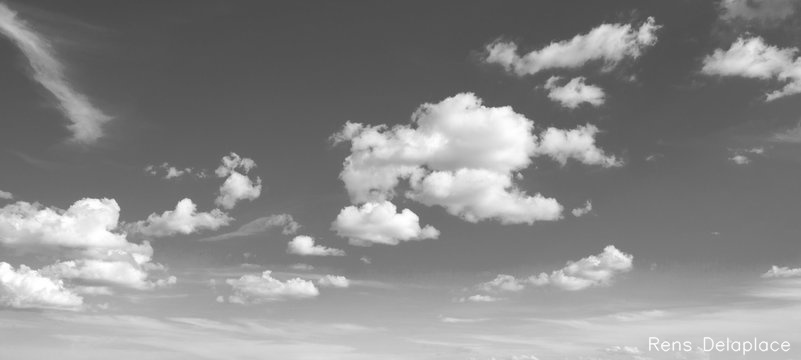
\includegraphics[keepaspectratio]{./out/assignement5.jpg}}
\caption{alt text}
\end{figure}

    \paragraph{Assignment 6}\label{assignment-6}

\begin{quote}
Threshold the grayscale image at 50\% of the maximum value for this
datatype.
\end{quote}

    \begin{tcolorbox}[breakable, size=fbox, boxrule=1pt, pad at break*=1mm,colback=cellbackground, colframe=cellborder]
\prompt{In}{incolor}{8}{\boxspacing}
\begin{Verbatim}[commandchars=\\\{\}]
\PY{c+c1}{\PYZsh{} Get the maximum pixel value for the datatype}
\PY{n}{max\PYZus{}value} \PY{o}{=} \PY{n}{np}\PY{o}{.}\PY{n}{iinfo}\PY{p}{(}\PY{n}{image}\PY{o}{.}\PY{n}{dtype}\PY{p}{)}\PY{o}{.}\PY{n}{max}
\PY{n}{threshold\PYZus{}value} \PY{o}{=} \PY{n}{max\PYZus{}value} \PY{o}{/}\PY{o}{/} \PY{l+m+mi}{2}  \PY{c+c1}{\PYZsh{} 50\PYZpc{} of max value}

\PY{n}{\PYZus{}}\PY{p}{,} \PY{n}{thresholded\PYZus{}image} \PY{o}{=} \PY{n}{cv2}\PY{o}{.}\PY{n}{threshold}\PY{p}{(}\PY{n}{grayscale\PYZus{}image}\PY{p}{,} \PY{n}{threshold\PYZus{}value}\PY{p}{,} \PY{l+m+mi}{255}\PY{p}{,} \PY{n}{cv2}\PY{o}{.}\PY{n}{THRESH\PYZus{}BINARY}\PY{p}{)}
\PY{n}{thresholded\PYZus{}image} \PY{o}{=} \PY{n}{add\PYZus{}name\PYZus{}to\PYZus{}image}\PY{p}{(}\PY{n}{thresholded\PYZus{}image}\PY{p}{)}
\PY{n}{cv2}\PY{o}{.}\PY{n}{imwrite}\PY{p}{(}\PY{l+s+s1}{\PYZsq{}}\PY{l+s+s1}{out/assignement6.jpg}\PY{l+s+s1}{\PYZsq{}}\PY{p}{,} \PY{n}{thresholded\PYZus{}image}\PY{p}{)}
\end{Verbatim}
\end{tcolorbox}

            \begin{tcolorbox}[breakable, size=fbox, boxrule=.5pt, pad at break*=1mm, opacityfill=0]
\prompt{Out}{outcolor}{8}{\boxspacing}
\begin{Verbatim}[commandchars=\\\{\}]
True
\end{Verbatim}
\end{tcolorbox}
        
    \begin{figure}
\centering
\pandocbounded{
\includegraphics[keepaspectratio]{./out/assignement6.jpg}}
\caption{alt text}
\end{figure}

    \paragraph{Assignment 7}\label{assignment-7}

\begin{quote}
Threshold the grayscale image at the ideal threshold determined by
Otsu's method.
\end{quote}

    \begin{tcolorbox}[breakable, size=fbox, boxrule=1pt, pad at break*=1mm,colback=cellbackground, colframe=cellborder]
\prompt{In}{incolor}{9}{\boxspacing}
\begin{Verbatim}[commandchars=\\\{\}]
\PY{n}{\PYZus{}}\PY{p}{,} \PY{n}{otsu\PYZus{}thresholded\PYZus{}image} \PY{o}{=} \PY{n}{cv2}\PY{o}{.}\PY{n}{threshold}\PY{p}{(}\PY{n}{grayscale\PYZus{}image}\PY{p}{,} \PY{l+m+mi}{0}\PY{p}{,} \PY{l+m+mi}{255}\PY{p}{,} \PY{n}{cv2}\PY{o}{.}\PY{n}{THRESH\PYZus{}BINARY} \PY{o}{+} \PY{n}{cv2}\PY{o}{.}\PY{n}{THRESH\PYZus{}OTSU}\PY{p}{)}

\PY{n}{otsu\PYZus{}thresholded\PYZus{}image} \PY{o}{=} \PY{n}{add\PYZus{}name\PYZus{}to\PYZus{}image}\PY{p}{(}\PY{n}{otsu\PYZus{}thresholded\PYZus{}image}\PY{p}{)}
\PY{n}{cv2}\PY{o}{.}\PY{n}{imwrite}\PY{p}{(}\PY{l+s+s1}{\PYZsq{}}\PY{l+s+s1}{out/assignement7.jpg}\PY{l+s+s1}{\PYZsq{}}\PY{p}{,} \PY{n}{otsu\PYZus{}thresholded\PYZus{}image}\PY{p}{)}
\end{Verbatim}
\end{tcolorbox}

            \begin{tcolorbox}[breakable, size=fbox, boxrule=.5pt, pad at break*=1mm, opacityfill=0]
\prompt{Out}{outcolor}{9}{\boxspacing}
\begin{Verbatim}[commandchars=\\\{\}]
True
\end{Verbatim}
\end{tcolorbox}
        
    \begin{figure}
\centering
\pandocbounded{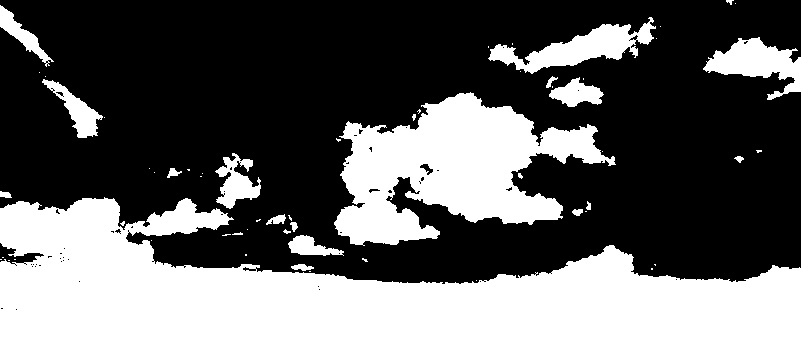
\includegraphics[keepaspectratio]{./out/assignement7.jpg}}
\caption{alt text}
\end{figure}

    \subsubsection{Exercise 3}\label{exercise-3}

\paragraph{Assignment 8}\label{assignment-8}

\begin{quote}
Adaptively threshold the grayscale version of painting2.jpg so you get a
similar result to the one below, where the background is uniformly white
and you can cut out the painting along black lines.
\end{quote}

    \begin{tcolorbox}[breakable, size=fbox, boxrule=1pt, pad at break*=1mm,colback=cellbackground, colframe=cellborder]
\prompt{In}{incolor}{10}{\boxspacing}
\begin{Verbatim}[commandchars=\\\{\}]
\PY{c+c1}{\PYZsh{} Read the image in grayscale}
\PY{n}{painting\PYZus{}image} \PY{o}{=} \PY{n}{cv2}\PY{o}{.}\PY{n}{imread}\PY{p}{(}\PY{l+s+s2}{\PYZdq{}}\PY{l+s+s2}{img/painting2.jpg}\PY{l+s+s2}{\PYZdq{}}\PY{p}{,} \PY{n}{cv2}\PY{o}{.}\PY{n}{IMREAD\PYZus{}GRAYSCALE}\PY{p}{)}

\PY{c+c1}{\PYZsh{} Ensure the image is in 8\PYZhy{}bit format}
\PY{n}{painting\PYZus{}image} \PY{o}{=} \PY{n}{cv2}\PY{o}{.}\PY{n}{convertScaleAbs}\PY{p}{(}\PY{n}{painting\PYZus{}image}\PY{p}{)}

\PY{n}{adaptive\PYZus{}thresholded\PYZus{}image} \PY{o}{=} \PY{n}{cv2}\PY{o}{.}\PY{n}{adaptiveThreshold}\PY{p}{(}\PY{n}{painting\PYZus{}image}\PY{p}{,} \PY{l+m+mi}{255}\PY{p}{,} \PY{n}{cv2}\PY{o}{.}\PY{n}{ADAPTIVE\PYZus{}THRESH\PYZus{}GAUSSIAN\PYZus{}C}\PY{p}{,} \PY{n}{cv2}\PY{o}{.}\PY{n}{THRESH\PYZus{}BINARY}\PY{p}{,} \PY{l+m+mi}{21}\PY{p}{,} \PY{l+m+mi}{10}\PY{p}{)}

\PY{n}{adaptive\PYZus{}thresholded\PYZus{}image} \PY{o}{=} \PY{n}{add\PYZus{}name\PYZus{}to\PYZus{}image}\PY{p}{(}\PY{n}{adaptive\PYZus{}thresholded\PYZus{}image}\PY{p}{)}
\PY{n}{cv2}\PY{o}{.}\PY{n}{imwrite}\PY{p}{(}\PY{l+s+s2}{\PYZdq{}}\PY{l+s+s2}{out/assignement8.jpg}\PY{l+s+s2}{\PYZdq{}}\PY{p}{,} \PY{n}{adaptive\PYZus{}thresholded\PYZus{}image}\PY{p}{)}
\end{Verbatim}
\end{tcolorbox}

            \begin{tcolorbox}[breakable, size=fbox, boxrule=.5pt, pad at break*=1mm, opacityfill=0]
\prompt{Out}{outcolor}{10}{\boxspacing}
\begin{Verbatim}[commandchars=\\\{\}]
True
\end{Verbatim}
\end{tcolorbox}
        
    \begin{figure}
\centering
\pandocbounded{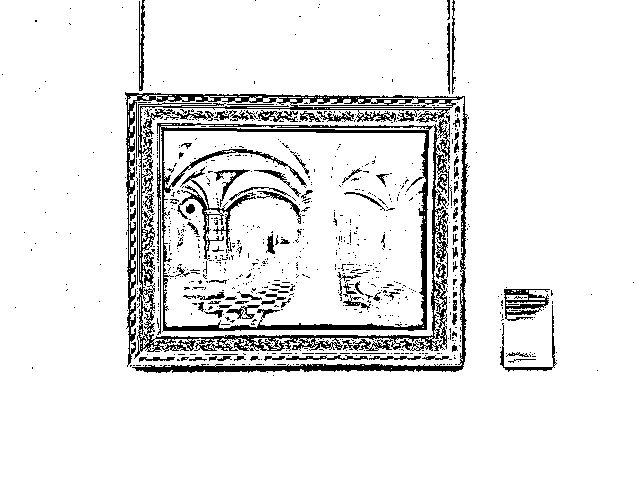
\includegraphics[keepaspectratio]{./out/assignement8.jpg}}
\caption{alt text}
\end{figure}

    \subsection{Filtering}\label{filtering}

    \subsubsection{Exercise 4}\label{exercise-4}

\paragraph{Assignment 9}\label{assignment-9}

\begin{quote}
Remove the white noise from whitenoise.png by Gaussian filtering. Find
parameters for the Gaussian kernel that you find strike a good balance
between noise level and blurriness of the result. This is subjective,
but experiment with it!
\end{quote}

    \begin{tcolorbox}[breakable, size=fbox, boxrule=1pt, pad at break*=1mm,colback=cellbackground, colframe=cellborder]
\prompt{In}{incolor}{11}{\boxspacing}
\begin{Verbatim}[commandchars=\\\{\}]
\PY{n}{whitenoise\PYZus{}image} \PY{o}{=} \PY{n}{cv2}\PY{o}{.}\PY{n}{imread}\PY{p}{(}\PY{l+s+s1}{\PYZsq{}}\PY{l+s+s1}{img/whitenoise.png}\PY{l+s+s1}{\PYZsq{}}\PY{p}{)}

\PY{n}{kernel\PYZus{}size} \PY{o}{=} \PY{p}{(}\PY{l+m+mi}{7}\PY{p}{,} \PY{l+m+mi}{7}\PY{p}{)}
\PY{n}{sigma} \PY{o}{=} \PY{l+m+mi}{4}
\PY{n}{gaussian\PYZus{}filtered\PYZus{}image} \PY{o}{=} \PY{n}{cv2}\PY{o}{.}\PY{n}{GaussianBlur}\PY{p}{(}\PY{n}{whitenoise\PYZus{}image}\PY{p}{,} \PY{n}{kernel\PYZus{}size}\PY{p}{,} \PY{n}{sigma}\PY{p}{)}

\PY{n}{gaussian\PYZus{}filtered\PYZus{}image} \PY{o}{=} \PY{n}{add\PYZus{}name\PYZus{}to\PYZus{}image}\PY{p}{(}\PY{n}{gaussian\PYZus{}filtered\PYZus{}image}\PY{p}{)}
\PY{n}{cv2}\PY{o}{.}\PY{n}{imwrite}\PY{p}{(}\PY{l+s+s1}{\PYZsq{}}\PY{l+s+s1}{out/assignement9.jpg}\PY{l+s+s1}{\PYZsq{}}\PY{p}{,} \PY{n}{gaussian\PYZus{}filtered\PYZus{}image}\PY{p}{)}
\end{Verbatim}
\end{tcolorbox}

            \begin{tcolorbox}[breakable, size=fbox, boxrule=.5pt, pad at break*=1mm, opacityfill=0]
\prompt{Out}{outcolor}{11}{\boxspacing}
\begin{Verbatim}[commandchars=\\\{\}]
True
\end{Verbatim}
\end{tcolorbox}
        
    \begin{figure}
\centering
\pandocbounded{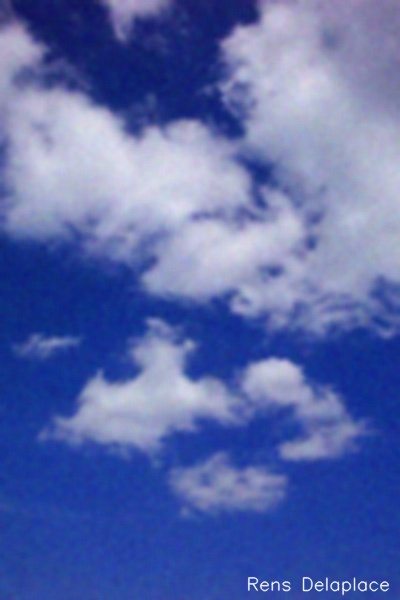
\includegraphics[keepaspectratio]{./out/assignement9.jpg}}
\caption{alt text}
\end{figure}

    \subsubsection{Question 2}\label{question-2}

\begin{quote}
Can you choose the kernel size and sigma of the distribution independent
of each other?
\end{quote}

The kernel size (the size of the filter window) and sigma (the standard
deviation of the Gaussian) are related.

If the kernel size is too small relative to sigma, important parts of
the Gaussian distribution will be cut off, reducing accuracy. If the
kernel size is too large, it increases computation time without
significantly improving the result. Kernel size is often chosen as a
multiple of sigma, for example 3*sigma. A larger kernel size generally
requires a larger sigma for effective smoothing. However, they can be
adjusted independently to find the right balance.

    \subsubsection{Exercise 5}\label{exercise-5}

\paragraph{Assignment 10}\label{assignment-10}

\begin{quote}
Test the Gaussian filter on saltandpeppernoise.png.
\end{quote}

    \begin{tcolorbox}[breakable, size=fbox, boxrule=1pt, pad at break*=1mm,colback=cellbackground, colframe=cellborder]
\prompt{In}{incolor}{12}{\boxspacing}
\begin{Verbatim}[commandchars=\\\{\}]
\PY{n}{saltpeppernoise\PYZus{}image} \PY{o}{=} \PY{n}{cv2}\PY{o}{.}\PY{n}{imread}\PY{p}{(}\PY{l+s+s1}{\PYZsq{}}\PY{l+s+s1}{img/saltandpeppernoise.png}\PY{l+s+s1}{\PYZsq{}}\PY{p}{)}

\PY{n}{kernel\PYZus{}size} \PY{o}{=} \PY{p}{(}\PY{l+m+mi}{7}\PY{p}{,} \PY{l+m+mi}{7}\PY{p}{)}
\PY{n}{sigma} \PY{o}{=} \PY{l+m+mi}{4}
\PY{n}{gaussian\PYZus{}filtered\PYZus{}image} \PY{o}{=} \PY{n}{cv2}\PY{o}{.}\PY{n}{GaussianBlur}\PY{p}{(}\PY{n}{saltpeppernoise\PYZus{}image}\PY{p}{,} \PY{n}{kernel\PYZus{}size}\PY{p}{,} \PY{n}{sigma}\PY{p}{)}

\PY{n}{gaussian\PYZus{}filtered\PYZus{}image} \PY{o}{=} \PY{n}{add\PYZus{}name\PYZus{}to\PYZus{}image}\PY{p}{(}\PY{n}{gaussian\PYZus{}filtered\PYZus{}image}\PY{p}{)}
\PY{n}{cv2}\PY{o}{.}\PY{n}{imwrite}\PY{p}{(}\PY{l+s+s1}{\PYZsq{}}\PY{l+s+s1}{out/assignement10.jpg}\PY{l+s+s1}{\PYZsq{}}\PY{p}{,} \PY{n}{gaussian\PYZus{}filtered\PYZus{}image}\PY{p}{)}
\end{Verbatim}
\end{tcolorbox}

            \begin{tcolorbox}[breakable, size=fbox, boxrule=.5pt, pad at break*=1mm, opacityfill=0]
\prompt{Out}{outcolor}{12}{\boxspacing}
\begin{Verbatim}[commandchars=\\\{\}]
True
\end{Verbatim}
\end{tcolorbox}
        
    \begin{figure}
\centering
\pandocbounded{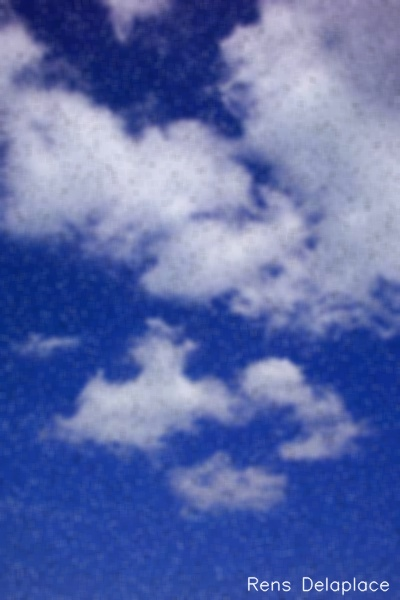
\includegraphics[keepaspectratio]{./out/assignement10.jpg}}
\caption{alt text}
\end{figure}

    \paragraph{Assignment 11}\label{assignment-11}

\begin{quote}
Apply median filtering on the same image.
\end{quote}

    \begin{tcolorbox}[breakable, size=fbox, boxrule=1pt, pad at break*=1mm,colback=cellbackground, colframe=cellborder]
\prompt{In}{incolor}{13}{\boxspacing}
\begin{Verbatim}[commandchars=\\\{\}]
\PY{n}{saltpeppernoise\PYZus{}image} \PY{o}{=} \PY{n}{cv2}\PY{o}{.}\PY{n}{imread}\PY{p}{(}\PY{l+s+s1}{\PYZsq{}}\PY{l+s+s1}{img/saltandpeppernoise.png}\PY{l+s+s1}{\PYZsq{}}\PY{p}{)}
\PY{n}{median\PYZus{}filtered\PYZus{}image} \PY{o}{=} \PY{n}{cv2}\PY{o}{.}\PY{n}{medianBlur}\PY{p}{(}\PY{n}{saltpeppernoise\PYZus{}image}\PY{p}{,} \PY{l+m+mi}{5}\PY{p}{)}

\PY{n}{median\PYZus{}filtered\PYZus{}image} \PY{o}{=} \PY{n}{add\PYZus{}name\PYZus{}to\PYZus{}image}\PY{p}{(}\PY{n}{median\PYZus{}filtered\PYZus{}image}\PY{p}{)}
\PY{n}{cv2}\PY{o}{.}\PY{n}{imwrite}\PY{p}{(}\PY{l+s+s1}{\PYZsq{}}\PY{l+s+s1}{out/assignement11.jpg}\PY{l+s+s1}{\PYZsq{}}\PY{p}{,} \PY{n}{median\PYZus{}filtered\PYZus{}image}\PY{p}{)}
\end{Verbatim}
\end{tcolorbox}

            \begin{tcolorbox}[breakable, size=fbox, boxrule=.5pt, pad at break*=1mm, opacityfill=0]
\prompt{Out}{outcolor}{13}{\boxspacing}
\begin{Verbatim}[commandchars=\\\{\}]
True
\end{Verbatim}
\end{tcolorbox}
        
    \begin{figure}
\centering
\pandocbounded{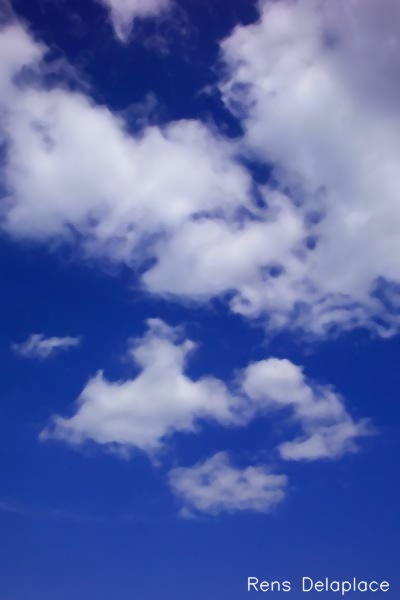
\includegraphics[keepaspectratio]{./out/assignement11.jpg}}
\caption{alt text}
\end{figure}

    \paragraph{Question 3}\label{question-3}

\begin{quote}
Which result is preferable and why?
\end{quote}

Median filtering is prefered for images with salt and pepper noise, as
it discards outliers (salt \& peper), while median filtering mixes these
values with the rest of the image.

    \subsubsection{Exercise 6}\label{exercise-6}

\paragraph{Assignment 12}\label{assignment-12}

\begin{quote}
Implement unsharp masking to sharpen unsharp.png. Make sure you do not
get overflow in your datatype!
\end{quote}

    \begin{tcolorbox}[breakable, size=fbox, boxrule=1pt, pad at break*=1mm,colback=cellbackground, colframe=cellborder]
\prompt{In}{incolor}{14}{\boxspacing}
\begin{Verbatim}[commandchars=\\\{\}]
\PY{n}{unsharp\PYZus{}image} \PY{o}{=} \PY{n}{np}\PY{o}{.}\PY{n}{float32}\PY{p}{(}\PY{n}{cv2}\PY{o}{.}\PY{n}{imread}\PY{p}{(}\PY{l+s+s1}{\PYZsq{}}\PY{l+s+s1}{img/unsharp.png}\PY{l+s+s1}{\PYZsq{}}\PY{p}{)}\PY{p}{)}

\PY{c+c1}{\PYZsh{} Blur the image}
\PY{n}{unsharp\PYZus{}image\PYZus{}float} \PY{o}{=} \PY{n}{unsharp\PYZus{}image}\PY{o}{.}\PY{n}{astype}\PY{p}{(}\PY{n}{np}\PY{o}{.}\PY{n}{float32}\PY{p}{)}
\PY{n}{blurred\PYZus{}image} \PY{o}{=} \PY{n}{cv2}\PY{o}{.}\PY{n}{GaussianBlur}\PY{p}{(}\PY{n}{unsharp\PYZus{}image\PYZus{}float}\PY{p}{,} \PY{p}{(}\PY{l+m+mi}{7}\PY{p}{,} \PY{l+m+mi}{7}\PY{p}{)}\PY{p}{,} \PY{l+m+mi}{4}\PY{p}{)}

\PY{c+c1}{\PYZsh{} Subtract the blurred from the original}
\PY{n}{difference\PYZus{}image} \PY{o}{=} \PY{n}{unsharp\PYZus{}image\PYZus{}float} \PY{o}{\PYZhy{}} \PY{n}{blurred\PYZus{}image}

\PY{c+c1}{\PYZsh{} Amplify the difference by multiplying it with a factor}
\PY{n}{amplified\PYZus{}difference} \PY{o}{=} \PY{n}{difference\PYZus{}image} \PY{o}{*} \PY{l+m+mf}{1.5}

\PY{c+c1}{\PYZsh{} Add this amplified difference image to the original image}
\PY{n}{sharpened\PYZus{}image} \PY{o}{=} \PY{n}{unsharp\PYZus{}image\PYZus{}float} \PY{o}{+} \PY{n}{amplified\PYZus{}difference}

\PY{n}{sharpened\PYZus{}image} \PY{o}{=} \PY{n}{np}\PY{o}{.}\PY{n}{clip}\PY{p}{(}\PY{n}{sharpened\PYZus{}image}\PY{p}{,} \PY{l+m+mi}{0}\PY{p}{,} \PY{l+m+mi}{255}\PY{p}{)}\PY{o}{.}\PY{n}{astype}\PY{p}{(}\PY{n}{np}\PY{o}{.}\PY{n}{uint8}\PY{p}{)}
\PY{n}{sharpened\PYZus{}image} \PY{o}{=} \PY{n}{add\PYZus{}name\PYZus{}to\PYZus{}image}\PY{p}{(}\PY{n}{sharpened\PYZus{}image}\PY{p}{)}
\PY{n}{cv2}\PY{o}{.}\PY{n}{imwrite}\PY{p}{(}\PY{l+s+s1}{\PYZsq{}}\PY{l+s+s1}{out/assignement12.jpg}\PY{l+s+s1}{\PYZsq{}}\PY{p}{,} \PY{n}{sharpened\PYZus{}image}\PY{p}{)}
\end{Verbatim}
\end{tcolorbox}

            \begin{tcolorbox}[breakable, size=fbox, boxrule=.5pt, pad at break*=1mm, opacityfill=0]
\prompt{Out}{outcolor}{14}{\boxspacing}
\begin{Verbatim}[commandchars=\\\{\}]
True
\end{Verbatim}
\end{tcolorbox}
        
    \begin{figure}
\centering
\pandocbounded{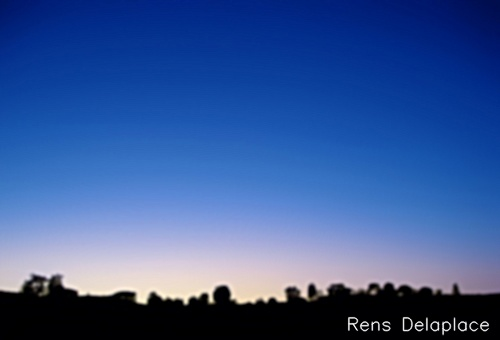
\includegraphics[keepaspectratio]{./out/assignement12.jpg}}
\caption{alt text}
\end{figure}

    \subsubsection{Exercise 7}\label{exercise-7}

\paragraph{Assignment 13}\label{assignment-13}

\begin{quote}
Write a program that blurs blots.png diagonally with the kernel below
(mind the multiplication factor in front).
\end{quote}

    \begin{tcolorbox}[breakable, size=fbox, boxrule=1pt, pad at break*=1mm,colback=cellbackground, colframe=cellborder]
\prompt{In}{incolor}{15}{\boxspacing}
\begin{Verbatim}[commandchars=\\\{\}]
\PY{n}{image} \PY{o}{=} \PY{n}{cv2}\PY{o}{.}\PY{n}{imread}\PY{p}{(}\PY{l+s+s2}{\PYZdq{}}\PY{l+s+s2}{img/blots.png}\PY{l+s+s2}{\PYZdq{}}\PY{p}{)}

\PY{n}{kernel} \PY{o}{=} \PY{p}{(}\PY{l+m+mi}{1}\PY{o}{/}\PY{l+m+mi}{7}\PY{p}{)} \PY{o}{*} \PY{n}{np}\PY{o}{.}\PY{n}{eye}\PY{p}{(}\PY{l+m+mi}{7}\PY{p}{,} \PY{n}{dtype}\PY{o}{=}\PY{n}{np}\PY{o}{.}\PY{n}{float32}\PY{p}{)}
\PY{n}{blurred\PYZus{}image} \PY{o}{=} \PY{n}{cv2}\PY{o}{.}\PY{n}{filter2D}\PY{p}{(}\PY{n}{image}\PY{p}{,} \PY{o}{\PYZhy{}}\PY{l+m+mi}{1}\PY{p}{,} \PY{n}{kernel}\PY{p}{)}

\PY{n}{blurred\PYZus{}image} \PY{o}{=} \PY{n}{add\PYZus{}name\PYZus{}to\PYZus{}image}\PY{p}{(}\PY{n}{blurred\PYZus{}image}\PY{p}{)}
\PY{n}{cv2}\PY{o}{.}\PY{n}{imwrite}\PY{p}{(}\PY{l+s+s2}{\PYZdq{}}\PY{l+s+s2}{out/assignement13.jpg}\PY{l+s+s2}{\PYZdq{}}\PY{p}{,} \PY{n}{blurred\PYZus{}image}\PY{p}{)}
\end{Verbatim}
\end{tcolorbox}

            \begin{tcolorbox}[breakable, size=fbox, boxrule=.5pt, pad at break*=1mm, opacityfill=0]
\prompt{Out}{outcolor}{15}{\boxspacing}
\begin{Verbatim}[commandchars=\\\{\}]
True
\end{Verbatim}
\end{tcolorbox}
        
    \begin{figure}
\centering
\pandocbounded{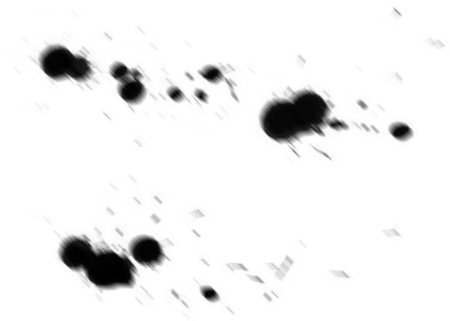
\includegraphics[keepaspectratio]{./out/assignement13.jpg}}
\caption{alt text}
\end{figure}


    % Add a bibliography block to the postdoc
    
    
    
\end{document}
